% Chapter 3

\chapter{Results and conclusion} % Write in your own chapter title
\label{Chapter3}

\indent In this section we will discuss results of different evaluations
and also how does our pipeline compares with others pipelines. From
figure ~\ref{bg_compare}, we can infer that Vibe is computationally very
efficient compared to other, therefore we select Vibe as background
subtraction algorithm in our final pipeline. We have seen different
skeleton output in figures ~\ref{contour_skeleton},
~\ref{morphological_skeleton}, ~\ref{dt_skeleton}, ~\ref{star_skeleton}.
We are targetting detection by skeleton motion. Use of star skeleton
would be the best choice to implement such detection method. Therefore
our final pipeline is based on Vibe as background subtracter and star
skeleton motion as detection feature. We have provided 'C' code for our
pipeline in apendix ~\ref{ApendixA}.

\indent We observe that with our implementation, code is able to detect
a moving person after it's 3 steps move. Figure  \ref{pipeline_images}
shows output images at different stages of pipeline.

\begin{figure}[!b]
\centering
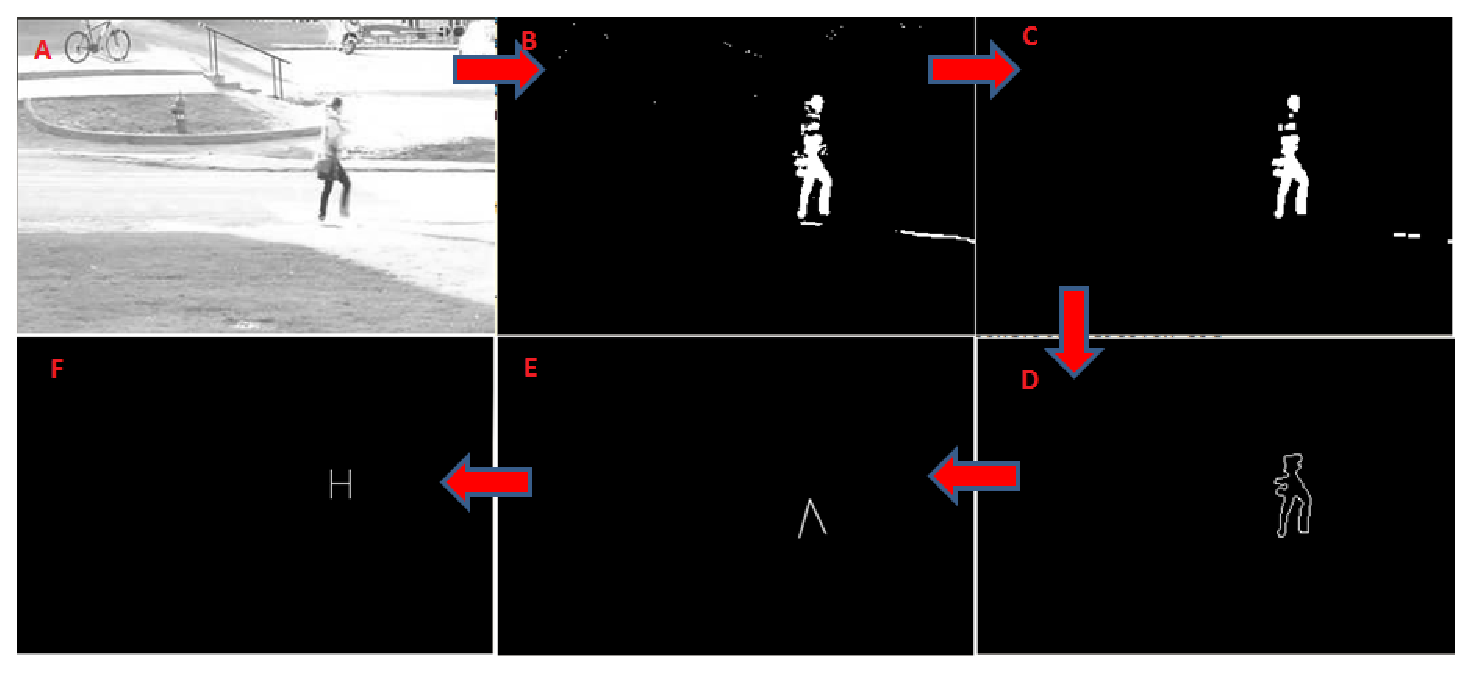
\includegraphics[height=200pt]{Figures/pipeline_images}
\caption{Images at different stage of pipeline. (From top left in
clockwise order) \textbf{a.} Gray Scale input frame to pipeline
\textbf{b.}Foreground extracted image using Vibe \textbf{c.} Cleaned
image \textbf{d.} Contour of moving object \textbf{e.} Plot of 3 points
of interest, centroid and two distance peaks nearer to bottom left and
bottom right corner of bounding box \textbf{f.} Virtual representation
of scene} 
\label{pipeline_images}
\end{figure}

\indent We have also done experiments with negative images like a person
moving on bicycle, or a vehicle moving on road. Our algorithm is
successfully able to reject these objects. Figure \ref{negative_inputs}
shows that how does this implementation rejects moving vehicle and
bicycle and  does not recognize them as human.
\begin{figure}[!b]
\centering
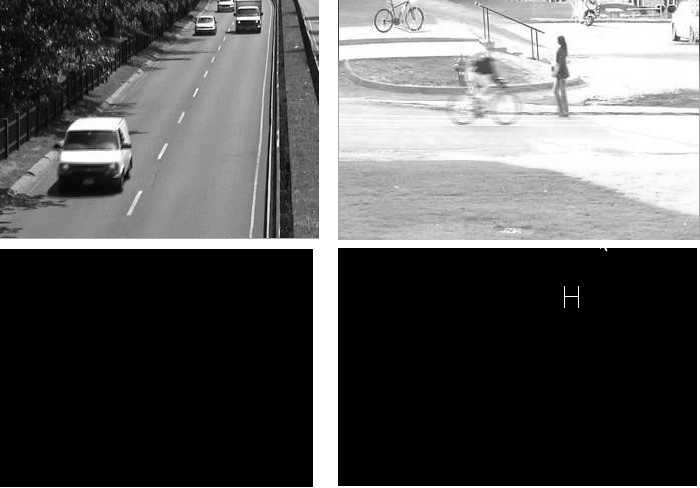
\includegraphics[height=300pt]{Figures/negative_inputs}
\caption{Input and output of pipeline in case of negative images}
\label{negative_inputs}
\end{figure}


\indent Comparison of proposed framework with HAAR and IDIAP (based on
covariance feature) detection algorithm in figure
\ref{pipeline_execution_time} shows that, this is quite faster. Our
pipeline takes just 3.6 mS on the average, while HARR and IDIAP takes
around 20mS and 248 mS respectively per frame. This timing was observed
with a system having DMIPS = 800.

\begin{figure}[!b]
\centering
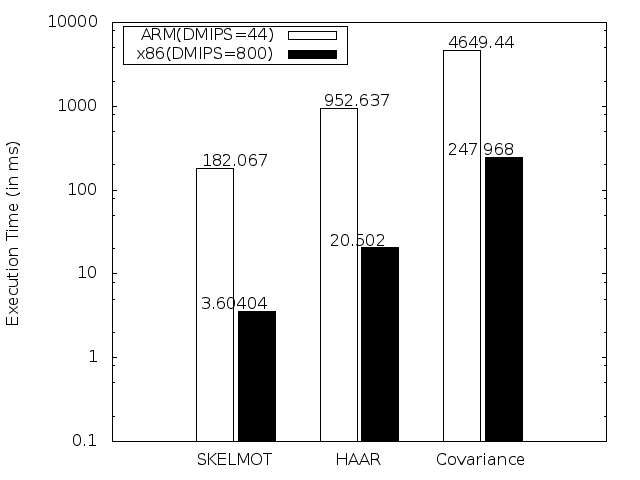
\includegraphics[height=300pt]{Figures/pipeline_execution_time}
\caption{Variation of different pipeline execution time with a system
having DMIPS=800}
\label{pipeline_execution_time}
\end{figure}

\indent We have also implemented above pipelines with ARM11 platform
with DMIPS = 44.  Comparison of timing at ARM11 platform has been shown
in figure \ref{arm11_pipeline_execution_time}. Our pipeline takes 182 ms
on the average, while HARR and IDIAP takes around 942ms and 4.65 s
respectively per frame. 

\begin{figure}[!h]
\centering
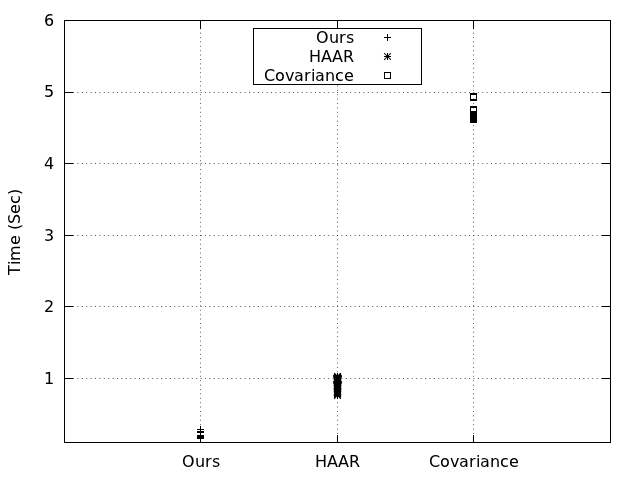
\includegraphics[height=300pt]{Figures/arm11_pipeline_execution_time}
\caption{Variation of different pipeline execution time with an ARM11 system
having DMIPS=44}
\label{arm11_pipeline_execution_time}
\end{figure}

\indent We have seen that method based on covariance or haar descriptor
is very slow in comparison with skeleton motion descriptor. Therefore,
if a surveillance application requires to identify moving person, then
we might not need to use complex algorithm to get real time performance
with low cost embedded platform. By using proposed algorithm, we can
save a lot of computational power. However, if we wish to detect human
from still frame, then we need to go for other methods. To use other
methods such as haar or covariance features based descriptor in real
time environment, we recommend to implement them in hardware. This
dedicated hardware can further be used with low end micro-controller to
achieve end result.
